 $\chapter{Diseño del sistema} $

Para realizar el procesamiento más adecuado al sistema, en primer lugar se tendrá que entrenar con una serie de señales obtenidas de prueba con tal fin. Una vez obtenidas estas señales de entrenamiento y desarrollado todo el algoritmo ya podremos testear que éste es correcto y cumple con su objetivo.  

\begin{figure}[H]
	\center
	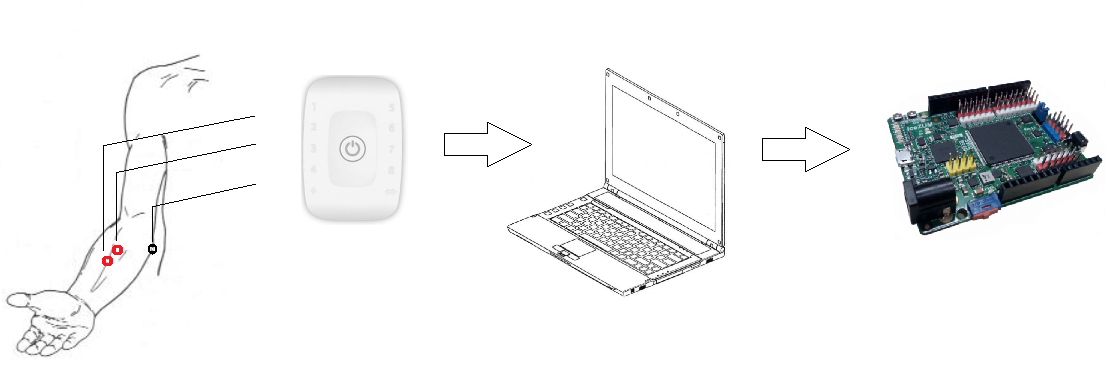
\includegraphics[scale=0.6]{imagenes/Disenodelsistema/sistema.png}
	\caption{Sistema}
	\label{fig:Sistema}
\end{figure}


El kit de Biosignalplux y sus electrodos nos permite adquirir las señales EMG de entrenamiento, que mediante Bluethooth son enviadas al ordenador en tiempo real y guardadas en el software OpenSignals. Estas señales que hemos guardado son posteriormente procesadas en Matlab para su filtrado y captación de parámetros que nos permitan distinguir los distintos estados en los que se encuentra el músculo.
 \newline
Una vez las señales son procesadas son enviadas mediante comunicación serie a la FPGA, en la que se va a definir el modo de control. 

En los siguientes capítulos vamos a ver más detenidamente todo el proceso de obtención así como las conclusiones del proyecto.

\section{Adquisición}
En la adquisición de señales EMG hay que tener en cuenta un correcto acondicionamiento de la piel.
\subsection{Preparación de la piel} \label{sec:Preparaciondelapiel}
 Es necesario a la hora de obtener señales EMG una correcta preparación de la piel dónde vamos a colocar los electrodos; de forma que la calidad de la señal obtenida sea la mejor posible. Para este propósito es recomendable usar un gel abrasivo o alcohol tanto para eliminar las células muertas de la piel como para reducir la sequedad de la misma. Tras la correcta limpieza con un paño suave se asegura que la zona quede totalmente limpia y seca. \newline
\subsection{Los electrodos} \label{sec:Loselectrodos}
Para ello se usan 3 electrodos  (2 y uno de referencia) que se colocan directamente sobre la piel y son capaces de captar la actividad bioeléctrica. La ubicación de los electrodos va a influir directamente sobre la calidad de las señales obtenidas; una correcta colocación sería en paralelo a las fibras musculares, en la zona central del músculo del que queramos obtener la actividad eléctrica. Estos deberán estar separados de 1 a 2 cm y el de referencia deberá estar colocado en un sitio dónde sepamos que la actividad será minima; en los tendones y el borde del músculo las fibras musculares se vuelven más delgadas y pequeñas por lo que son el sitio ideal para colocar el electrodo de referencia. 

Antes de colocar los electrodos se puede usar una pasta conductiva que mejora considerablemente la captación de estos de las señales.\newline

\begin{figure}[H]
	\center
	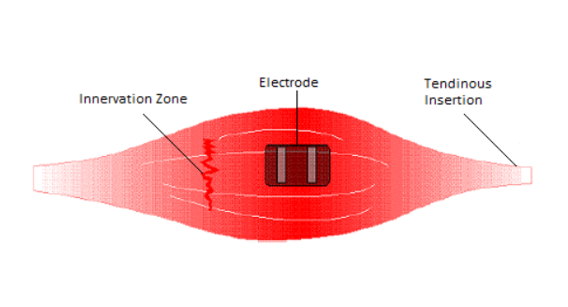
\includegraphics[scale=0.8]{imagenes/Disenodelsistema/electrodo.png}
	\caption{Posición de los electrodos}
	\label{fig:Posicion}
\end{figure}

\subsection{Obtención de señales}

Con lo visto en \ref{sec:Preparaciondelapiel} y \ref{sec:Loselectrodos} tendríamos que definir el músculo que va a hacer de instrumento de control para el sistema. Se plantea la idea de usar un músculo del antebrazo por la facilidad para la colocación de los electrodos, así como a la hora de descriminar los distintos movimientos que nos van a permitir el control del sistema. Un correcto sitio sería con los 2 electrodos en la parte central y el de referencia en el codo que es un punto con poca actividad eléctrica.\newline 

El músculo flexor del carpo (figura \ref{fig:flexor}) será  el que eligiremos debido a su posición central, ya que permite contraerlo y relajarlo con facilidad. \newline Por lo tanto este será el músculo sobre el cual vamos a colocar los electrodos para realizar la toma de señales y empezar a discriminar los distintos movimientos. Las pruebas deberán hacerse para los dos brazos, ya que nos permitirá más grados de libertad a la hora de elegir el método de control del sistema.  

\begin{figure}[H]
	\center
	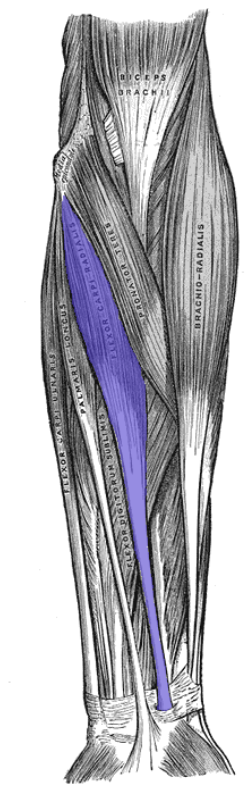
\includegraphics[scale=0.5]{imagenes/Disenodelsistema/flexor.png}
	\caption{Músculo flexor del carpo en el antebrazo}
	\label{fig:flexor}
\end{figure}


Se tomarán unas señales EMG de entrenamiento, que mediante Bluethooth son enviadas al ordenador en tiempo real y vistas en el software OpenSignals. Desde que ponemos en marcha el programa hasta que lo paramos las señales EMG captadas con los electrodos se pueden ver en el mismo programa,y elegir el rango de tiempo que queremos guardar. Estas señales son guardadas como archivos de texto (.txt) dónde se guarda el número de muestra y su valor correspondiente.\newline


\begin{figure}[H]
	\center
	\includegraphics[scale=0.3]{imagenes/Disenodelsistema/Ejemplo.png}
	\caption{Señal EMG captada por OpenSignals}
	\label{fig:Ejemplo}
\end{figure}

En la figura \ref{fig:Ejemplo} se puede distinguir bastante bien las diferentes contracciones que ha sufrido el músculo en el proceso de obtención. Las zonas con una menor amplitud se tratan de relajaciones o momentos en los que el flexor se encuentra relajado y con poca actividad eléctrica. En el momento en el que contraemos voluntariamente el músculo se alcanzan picos de gran amplitud; estas amplitudes serán las que el algoritmo tenga que discriminar para determinar si el músculo se encuentra relajado o contraído.
Tras la obtención, un procesamiento con Matlab será necesario para acondicionarlas y preparar las señales para su uso.


\subsection{Procesamiento en Matlab}

A la hora de trabajar con bioseñales para el control de mecanismos robóticos, se necesitan señales sin interferencias. Las interferencias más comunes,como hemos visto en \ref{sec:Ruido} es el ruido de 50Hz de la red eléctrica; aunque también existen de otro tipo como las que ocurren en la medición, como el movimiento de los cables o incluso los problemas del mismo equipo que hace las medidas. Para realizar el procesamiento digital de la señal EMG por lo tanto, será necesario tener en cuenta que la mayor parte de su información se encuentra en el rango de frencuencias de 5Hz a 500Hz. Además debido a su comportamiento no determinista, debe procesarse con técnicas de caracterización que permitan conocer características definidas de la señal, a través de las cuales apicar los determinados métodos de control. \newline

Las señales en formato .txt son cargadas en Matlab mediante la función dlmread, que lee los datos del fichero y los guarda en una matriz, donde el valor de la frecuencia de muestreo de la señal se almacena en una variable.  La expresión matemática se define en

\begin{equation}
I = K * dT^{0.44}*(W*H)^{0.725}
EMG(V)=\frac{((ADC/2^n)-1/2)*Vcc)/G}

\end{equation}

\begin{itemize}
	\item I = Max. Intensity (A).
	\item dT =Temperature rise over ambient (Cº)
	\item W,H = With and Height (mils)
	\item K = 0.024 for internal traces and 0.048 for external traces.
\end{itemize}

